\chapter{Integrating Fetch and Decode}

\section{Integration}
We now have working Fetch, Decode, and Execute modules.  Now it is time to put them together to produce a system that can:
\begin{enumerate}
	\item Update the program counter
	\item Read the appropriate instruction from the instruction datafile
	\item Read the correct registers
	\item Update all control lines
	\item Sign extend address data
	\item Calculate Branch Target Addresses
	\item Provide a zero bit for conditional branch instructions
	\item Produce ALU results for R-Type and D-Type instructions
\end{enumerate}

Once we can do all of this, we will be ready for the iMemory stage.  We currently have the fetch and decode module integrated into fd\_integration.sv.  We also have a working execute module.  Today we need to integrate the execute module with the fetch and decode stages.  The new testbench should be called fde\_integration.sv.  Please reuse the instructions from your Expected Results Table that you used when you integrated fetch and decode.  Once integrated, you should be able to produce a simulation that includes the outputs of fetch and decode as well as 3 new outputs from execute:
\begin{enumerate}
	\item Branch Target
	\item ALU Result
	\item Zero
\end{enumerate}   

These three new outputs are marked on Figure Figure ~\ref{fig:integrated_execute}.  To verify these outputs, you should have already  updated the Expected Results Table to include these three outputs.  To test this integration, I recommend copying the contents of fd\_integration.sv into fde\_integration.sv and then modifying from there, adding your execute module, cr values, verify statements, etc that are necessary to verify the integration of the execute module. fd\_integration had 139 test cases, so fde\_integration should have 159 test cases.

\begin{figure}
	\caption{Execute Stage}\label{fig:integrated_execute}
	\begin{center}
		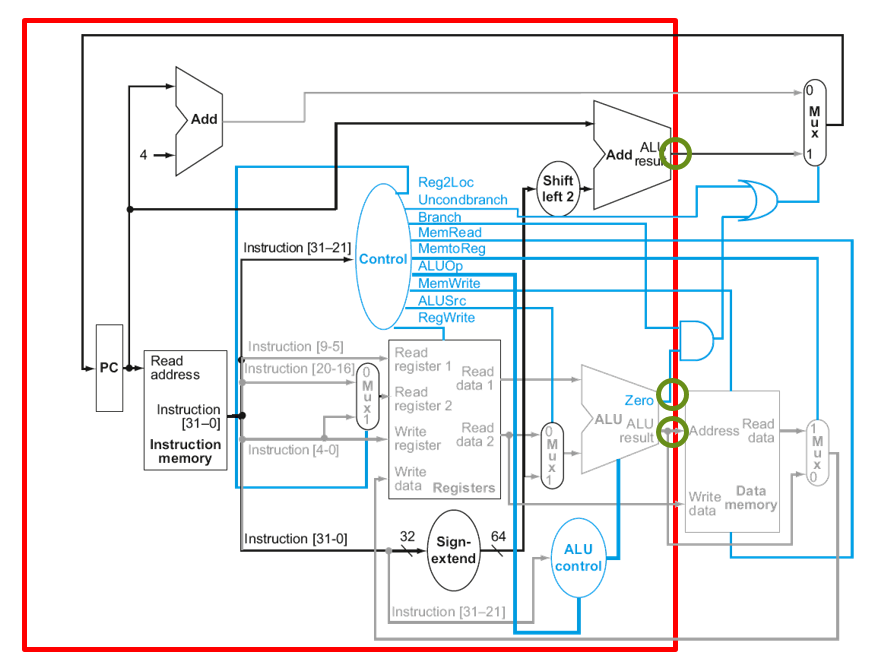
\includegraphics[width=4.75in]{../images/integrated_execute.png}
	\end{center}
\end{figure} 

\section{Your Assignment}

You are to:
\begin{enumerate}
\item Create fde\_integration.sv
\item Verify that your simulation results match your expected results.
\item Rather than writing a lab report, please produce a landscape mode PDF file called Lab10\_lastname.pdf that includes (in this order):
\begin{enumerate}
	\item Your name and the lab number.
	\item A snip of your completed Expected Results Table.
	\item A snip of the Simulation Results for the iExecute test.  Please show instructions in hex, opcodes and control signals in binary and everything else in signed decimal.  
	\item Copy and paste the entire log from BEGIN TEST RESULTS to END TEST RESULTS into your file.  The results have gotten too long to use the snipping tool.	
\end{enumerate}
\item Upload Lab10\_lastname.pdf file to Canvas.
\item Zip up your ARM-Lab directory and submit it on Canvas as well.  I will run your code against my correct testbench to verify that your code and testbench work correctly.
\end{enumerate}